\chapter{Problema dei cammini minimi - Floyd-Warshall}
Come al solito diamo qualche definizione per poter lavorare successivamente in maniera
agile.
\section{Definizioni}
\subsection{Grafo}
Un Grafo viene definito come $G=(V,E)$ dove:
\begin{itemize}
    \item $V = \{v_1,v_2,v_3,...,v_n\}$ insieme di vertici
    \item $E= \{e_1,e_2,e_3,...,e_m\}$ insieme di archi
\end{itemize}
\paragraph*{Dimensione di G} $\rightarrow$ (n,m).
Arco $e_k \rightarrow$ relazione R tra due vertici $v_i$ e $v_j$
\paragraph*{R può essere}
\begin{itemize}
    \item Simmetrica - Grafo NON Orientato - cioè $v_i \, R \, v_j \Leftrightarrow v_j \, R \, v_i$
    \item Asimmetrica - Grafo Orientato (o diretto) - cioè $v_i \, R \, v_j \nLeftrightarrow  v_j \, R \, v_i$
\end{itemize}
Un grafo orientato è caratterizzato da un verso di percorrenza degli archi unidirezionale.
In questo caso E è sottoinsieme di $V^2$.
\begin{center}
    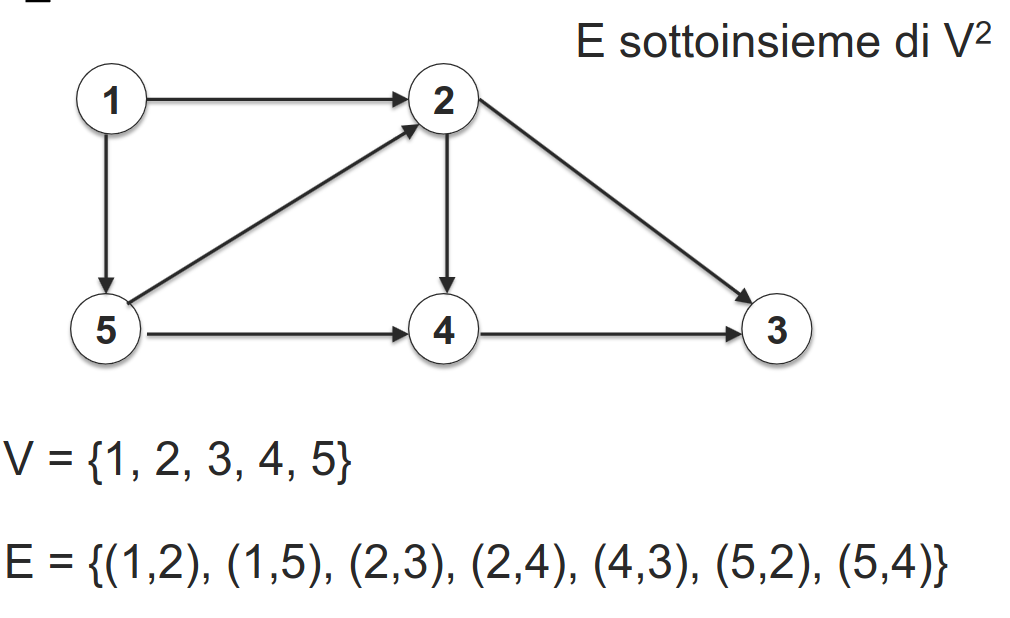
\includegraphics[width=80mm, scale=0.5]{grafo_orientato.png}
\end{center}
\begin{center}
    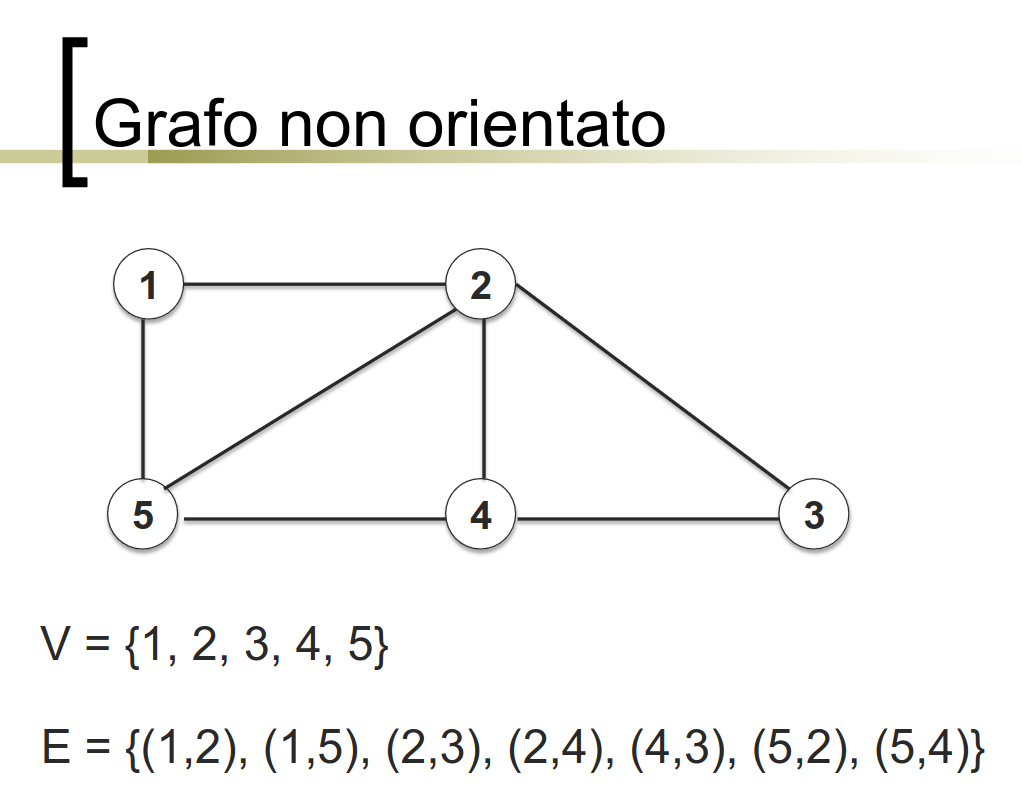
\includegraphics[width=80mm, scale=0.5]{grafo_non_orientato.png}
\end{center}
\subsection{Adiacenza}
Un vertifica v è adiacente a un vertice u se $(u,v)\in E$.\\
Per esempio nella rappresentazione del grafo orientato il vertice \textbf{1} è adiacante ai
vertici \textbf{2 e 5}, infatti notiamo che in E è presente $(1,2), (1,5)$.
\subsection{Rappresentazione di un grafo}
Abbiamo 2 rappresentazioni possibili:
\begin{itemize}
    \item Liste di adiacenza
    \item Matrice di adiacenza
\end{itemize}
